\documentclass[11pt,a4paper]{article}

\usepackage[T1]{fontenc}
\usepackage[utf8]{inputenc}
\usepackage{lmodern}
\usepackage[margin=2.5cm]{geometry}
\usepackage{amsmath,amssymb}
\usepackage{microtype}
\usepackage{hyperref}
\usepackage{listings}
\usepackage{xcolor}
\usepackage{booktabs}
\usepackage{array}
\usepackage{enumitem}
\usepackage{tikz}
\usetikzlibrary{positioning,shapes.geometric,arrows.meta}
\usepackage{parskip}

\hypersetup{
  colorlinks=true,
  linkcolor=black,
  urlcolor=blue!60!black,
  citecolor=black
}

% Java code listing style
\lstdefinestyle{java}{
  language=Java,
  basicstyle=\ttfamily\footnotesize,
  keywordstyle=\bfseries\color{blue!70!black},
  commentstyle=\itshape\color{gray},
  stringstyle=\color{orange!80!black},
  numberstyle=\tiny\color{gray},
  numbers=left,
  numbersep=8pt,
  frame=single,
  framesep=4pt,
  rulecolor=\color{black!20},
  backgroundcolor=\color{black!3},
  breaklines=true,
  breakatwhitespace=false,
  tabsize=4,
  showstringspaces=false,
  xleftmargin=14pt,
  xrightmargin=4pt,
  aboveskip=8pt,
  belowskip=8pt,
}

\lstset{style=java}

\title{\textbf{ExactPoly: A Java Library for Exact Symbolic\\
Polynomial Arithmetic over the Rationals}}

\author{
  Trinsit W.\\
  \small Independent Researcher\\
  \small \href{https://github.com/trinsitw}{https://github.com/trinsitw}
}

\date{May 2026}

\begin{document}

\maketitle

\begin{abstract}
We describe \textsc{ExactPoly}, a Java library for exact symbolic arithmetic
on univariate and multivariate polynomials with rational coefficients.
The library emerged as a reusable artifact from a study of a recursive identity
for power sums~\cite{trinsit2026}, and is general-purpose in design.
All polynomial coefficients are represented as exact rational numbers,
ensuring that no rounding error is introduced across recursive computations.
A key capability is \emph{polynomial composition}: the substitution of a
variable with another polynomial, yielding a new polynomial in closed symbolic
form. We describe the architecture of the five core classes, their design
properties, and demonstrate the library through worked examples drawn from
combinatorics, number theory, and symbolic computation.
\end{abstract}

\smallskip
\noindent\textbf{Keywords:} ExactPoly, symbolic computation, polynomial arithmetic,
exact arithmetic, rational numbers, computer algebra, Java.

\bigskip
\hrule

%----------------------------------------------------------------------
\section{Introduction}
%----------------------------------------------------------------------

Exact symbolic polynomial computation is a foundational capability in computer
algebra. Systems such as Mathematica and SymPy provide polynomial arithmetic as
part of larger ecosystems, but standalone, dependency-free implementations in
Java --- particularly those that maintain exact rational arithmetic throughout
--- are less common.

This library, named \textbf{ExactPoly}, was developed alongside a study of a
recursive identity for the power sum
$S(k,n)=\sum_{i=1}^{n}i^{k}$~\cite{trinsit2026}.
During that work it became apparent that the polynomial manipulation routines
had value independently of the problem that motivated them, and warranted
separate documentation.

The library provides five core classes:
\begin{itemize}[noitemsep]
  \item \texttt{RationalNumber}: arbitrary-precision rational arithmetic,
  \item \texttt{IndeterminateExponent}: a variable--exponent pair,
  \item \texttt{MultivariateMonomial}: a rational coefficient times a product of variables,
  \item \texttt{MultivariatePolynomial}: a sum of multivariate monomials,
  \item \texttt{RationalPolynomial}: a dense univariate polynomial with division.
\end{itemize}

No floating-point arithmetic is introduced at any stage.
All intermediate and final results are exact.

%----------------------------------------------------------------------
\section{Library Architecture}
%----------------------------------------------------------------------

Figure~\ref{fig:classdiagram} shows the relationships among the five core
classes. \texttt{RationalNumber} is the foundational value type used throughout;
\texttt{IndeterminateExponent} and \texttt{MultivariateMonomial} build upward
toward \texttt{MultivariatePolynomial}, while \texttt{RationalPolynomial}
provides a parallel univariate track optimised for division.

\begin{figure}[h]
\centering
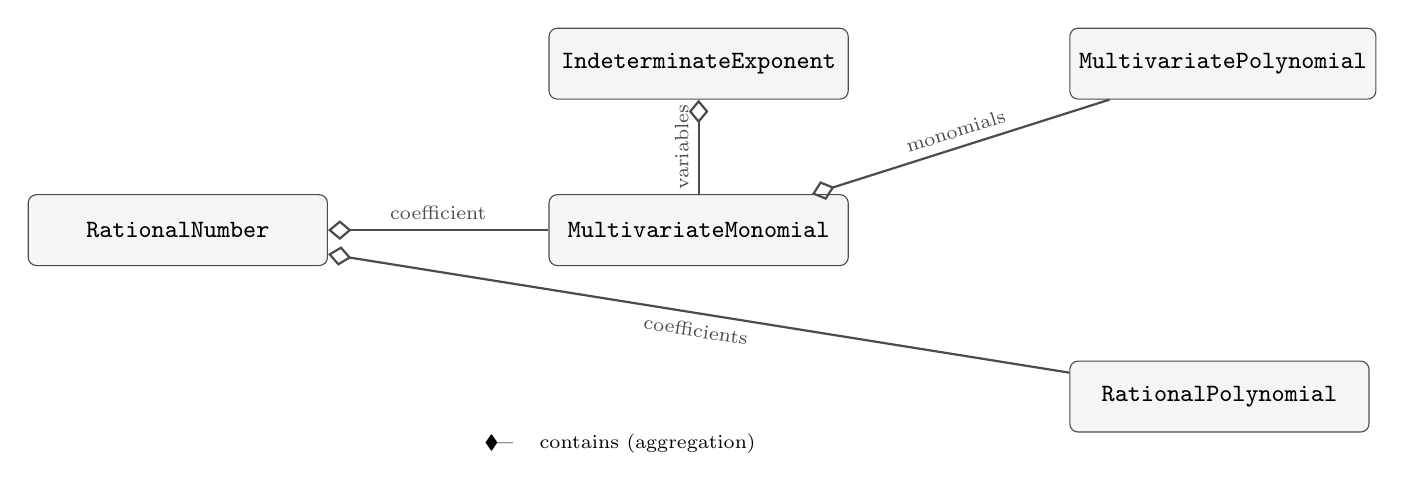
\begin{tikzpicture}[
  classbox/.style={
    rectangle, draw=black!70, rounded corners=3pt,
    fill=black!4, text centered,
    minimum width=3.8cm, minimum height=0.9cm,
    font=\ttfamily\small
  },
  uses/.style={-{Latex[length=2mm]}, dashed, thick, black!60},
  contains/.style={-{Diamond[open,length=3mm,width=2.5mm]}, thick, black!70},
  node distance=1.5cm and 2.8cm
]

% Nodes
\node[classbox] (rn)  {RationalNumber};
\node[classbox, above right=1.2cm and 2.8cm of rn] (ie)  {IndeterminateExponent};
\node[classbox, right=2.8cm of rn]  (mm)  {MultivariateMonomial};
\node[classbox, above right=1.2cm and 2.8cm of mm] (mp)  {MultivariatePolynomial};
\node[classbox, below right=1.2cm and 2.8cm of mm] (rp)  {RationalPolynomial};

% RationalNumber -> IndeterminateExponent (no direct link, just used)
% RationalNumber used by MultivariateMonomial
\draw[contains] (mm) -- node[above, font=\scriptsize, sloped]{coefficient} (rn);

% IndeterminateExponent contained in MultivariateMonomial
\draw[contains] (mm) -- node[above, font=\scriptsize, sloped]{variables} (ie);

% MultivariateMonomial contained in MultivariatePolynomial
\draw[contains] (mp) -- node[above, font=\scriptsize, sloped]{monomials} (mm);

% RationalPolynomial uses RationalNumber
\draw[contains] (rp) -- node[below, font=\scriptsize, sloped]{coefficients} (rn);

% Legend
\node[below=2.0cm of mm, xshift=-1.0cm, font=\scriptsize] (leg) {
  \begin{tabular}{ll}
    $\blacklozenge$\!\!---\!\!\ & contains (aggregation) \\
  \end{tabular}
};

\end{tikzpicture}
\caption{Class relationships in ExactPoly. Diamond-end arrows indicate
aggregation: the tail class holds instances of the head class.
\texttt{MultivariatePolynomial} and \texttt{RationalPolynomial} provide
parallel tracks for multivariate and univariate computation respectively.}
\label{fig:classdiagram}
\end{figure}

\subsection{\texttt{RationalNumber}}

The foundational type. Internally stores numerator and denominator as
\texttt{BigInteger}, reduced to lowest terms at construction time.
The sign is normalised so the denominator is always positive.
The four arithmetic operations and integer exponentiation are supported.

Key design properties:
\begin{itemize}[noitemsep]
  \item \textit{Immutable value type.} Every operation returns a new instance;
        no mutation occurs.
  \item \textit{Automatic reduction.} The GCD is computed and divided out at
        construction, eliminating the need for a separate normalisation step.
  \item \textit{Equality by value.} \texttt{equals} implements the mathematical
        criterion $a/b = c/d \iff ad = bc$.
\end{itemize}

Constants \texttt{ZERO} and \texttt{ONE} are provided as static fields.

\subsection{\texttt{IndeterminateExponent}}

A pair \texttt{(char indeterminate, int exponent)} representing a single
variable raised to a positive integer power, e.g.\ $x^{3}$ or $n^{2}$.
Indeterminates are restricted to lowercase letters \texttt{a}--\texttt{z}.
The class implements \texttt{Comparable\textless{}IndeterminateExponent\textgreater{}}
by variable name, enabling canonical ordering within monomials.

\subsection{\texttt{MultivariateMonomial}}

A product of a \texttt{RationalNumber} coefficient and a list of
\texttt{IndeterminateExponent} factors, representing terms such as
$\tfrac{3}{2}x^{2}y^{3}$.
The constructor normalises the variable list into sorted canonical order and
collapses the zero-coefficient case to an empty variable list.

Multiplication of two monomials merges their variable lists by grouping on the
variable name and summing exponents.
The \texttt{indeterminateExponentList()} accessor returns a defensive copy,
preventing external mutation of internal state.

\subsection{\texttt{MultivariatePolynomial}}

A sum of \texttt{MultivariateMonomial} terms.
The constructor automatically combines like terms (monomials sharing the same
variable signature) and eliminates zero terms, maintaining a canonical form at
all times.

Supported operations include \texttt{add}, \texttt{subtract}, \texttt{multiply},
\texttt{pow}, \texttt{evaluate}, and \texttt{commonDenominatorForm}.
The most distinctive operation is \texttt{compose}, described separately below.

\subsection{Polynomial Composition}

The \texttt{compose(char\,t,\;MultivariatePolynomial\,s)} method substitutes
every occurrence of the indeterminate~$t$ in a polynomial~$p$ with a
polynomial~$s$, returning the result as a new \texttt{MultivariatePolynomial}.
Formally, if $p$ is a polynomial in variables including~$t$, then
\[
  \texttt{p.compose}(t,\, s) \;=\; p\bigl[\,t \mapsto s\,\bigr],
\]
which is itself a polynomial in the remaining variables and the variables of~$s$.

This elevates polynomials from passive data structures to \emph{first-class
functions}: instead of evaluating $p$ at a number, \texttt{compose} evaluates
$p$ at another polynomial and returns an exact symbolic result.
The operation is safe because all types in ExactPoly are immutable --- the
substitution produces a fresh object and leaves~$p$ and~$s$ unchanged.

\textbf{Role in power-sum computation.}
\texttt{compose} is the mechanism that makes the recursive power-sum algorithm
in~\cite{trinsit2026} work.
The identity requires evaluating $S(k-2,\,i-1)$, i.e.\ the already-derived
polynomial for $S(k-2,n)$ with $n$ replaced by $i-1$.
This is expressed directly as:
\[
  S(k{-}2,\, i{-}1) \;=\; \texttt{Sk2.compose('n',\; iMinus1)}
\]
where \texttt{iMinus1} is the polynomial $i - 1$.
The result is a symbolic polynomial in~$i$ that can then be multiplied,
summed, and processed further --- all without leaving the symbolic domain.
Without \texttt{compose}, this step would require either a numeric approximation
or a fundamentally different algorithm.

\textbf{Broader applicability.}
Beyond the motivating application, \texttt{compose} enables a range of symbolic
tasks: computing $p(n+1)-p(n)$ to verify telescoping identities,
constructing shifted polynomials $p(x-a)$ for change-of-variable arguments,
and building higher-order expressions by functional substitution.

\subsection{\texttt{RationalPolynomial}}

A dense univariate polynomial stored as a coefficient array indexed by degree.
Supports \texttt{add}, \texttt{subtract}, \texttt{multiply}, \texttt{pow},
scalar \texttt{divide}, \texttt{evaluate} via Horner's method, and polynomial
long division returning \texttt{[quotient, remainder]}.

\texttt{RationalPolynomial} is suited to problems where a single variable is
known in advance and division is required;
\texttt{MultivariatePolynomial} is suited to problems involving several
variables or polynomial composition.

%----------------------------------------------------------------------
\section{Design Properties}
%----------------------------------------------------------------------

Two properties follow directly from the implementation and are worth stating
explicitly.

\textbf{Canonical form.}
Every \texttt{MultivariatePolynomial} instance is in canonical form: like terms
are combined, zero terms are absent, and monomials are sorted by total degree
in descending order.
This is enforced in the constructor via \texttt{groupingBy} on the variable
signature, followed by filtering and sorting.
Since all operations return new instances through the same construction path,
the invariant is preserved throughout.
As a consequence, two instances represent the same polynomial if and only if
they are structurally equal, and \texttt{equals} is a simple set comparison on
monomials.

\textbf{Immutability and composition safety.}
Every type in ExactPoly is immutable: \texttt{RationalNumber},
\texttt{IndeterminateExponent}, \texttt{MultivariateMonomial}, and
\texttt{MultivariatePolynomial} all return new instances from every operation,
and all list accessors return defensive copies.
This is not merely a stylistic choice --- it is a prerequisite for
\texttt{compose} to be correct.
Polynomial composition substitutes a variable with a polynomial and uses
both the original and the substitution in subsequent reductions.
If any operand were mutable, a modification made during the substitution
could silently corrupt a memoised intermediate result, producing incorrect
output that is difficult to detect and reproduce.
Immutability guarantees that \texttt{compose} is referentially transparent:
the same inputs always produce the same output, regardless of what other
computations are in progress.


No \texttt{RationalNumber} operation introduces rounding error.
All arithmetic is performed on \texttt{BigInteger} numerators and denominators,
with GCD reduction at each construction step.
Integer overflow is impossible since \texttt{BigInteger} is unbounded.
This property is what makes the library suitable for deep recursive computations
such as the power-sum derivation in~\cite{trinsit2026}, where floating-point
error would accumulate across many levels.

%----------------------------------------------------------------------
\section{Example Applications}
%----------------------------------------------------------------------

\subsection{Verifying the Closed Form for $S(2,n)$}

The classical formula
$S(2,n)=\tfrac{1}{3}n^{3}+\tfrac{1}{2}n^{2}+\tfrac{1}{6}n$
can be constructed and numerically verified:

\begin{lstlisting}
MultivariatePolynomial S2 = new MultivariatePolynomial(
    new MultivariateMonomial(new RationalNumber(1, 3), 'n', 3),
    new MultivariateMonomial(new RationalNumber(1, 2), 'n', 2),
    new MultivariateMonomial(new RationalNumber(1, 6), 'n', 1)
);

// S(2,4) = 1 + 4 + 9 + 16 = 30
System.out.println(S2.evaluate(BigInteger.valueOf(4))); // 30
\end{lstlisting}

\subsection{Polynomial Composition: Telescoping and Recursive Substitution}

\texttt{compose} treats a polynomial as a function and evaluates it at
another polynomial, returning an exact symbolic result.
Two uses are illustrated here.

\textbf{Telescoping verification.}
A closed-form candidate $p(n)$ for $S(k,n)$ must satisfy
$p(n+1)-p(n)=(n+1)^{k}$.
For $S(1,n)=\tfrac{1}{2}n^{2}+\tfrac{1}{2}n$, we expect
$p(n+1)-p(n)=n+1$:

\begin{lstlisting}
MultivariatePolynomial p = new MultivariatePolynomial(
    new MultivariateMonomial(new RationalNumber(1, 2), 'n', 2),
    new MultivariateMonomial(new RationalNumber(1, 2), 'n', 1)
);

// Substitute n -> (n + 1)
MultivariatePolynomial nPlus1 = new MultivariatePolynomial(
    new MultivariateMonomial(new RationalNumber(1), 'n', 1),
    new MultivariateMonomial(new RationalNumber(1))
);

// p(n+1) - p(n) should equal (n+1)
MultivariatePolynomial diff = p.compose('n', nPlus1).subtract(p);
System.out.println(diff); // (1)(n^1) + (1)   i.e. n+1  [correct]
\end{lstlisting}

\textbf{Recursive substitution in power-sum derivation.}
The recursive identity for $S(k,n)$~\cite{trinsit2026} requires forming
$S(k{-}2,\,i{-}1)$: the polynomial for the lower-order sum, with $n$ replaced
by $i-1$.
\texttt{compose} produces this in one call, returning a symbolic polynomial
in~$i$ ready for further arithmetic:

\begin{lstlisting}
// Sk2 is the already-derived MultivariatePolynomial for S(k-2, n)
// Substitute n -> (i - 1)
MultivariatePolynomial iMinus1 = new MultivariatePolynomial(
    new MultivariateMonomial(new RationalNumber(1), 'i', 1),
    new MultivariateMonomial(new RationalNumber(-1))
);

MultivariatePolynomial Sk2AtIMinus1 = Sk2.compose('n', iMinus1);
// Result: S(k-2, i-1) as a polynomial in i, exact, ready to sum
\end{lstlisting}

Without \texttt{compose}, this step would require a numeric approximation or
a fundamentally different algorithm.
The result remains fully symbolic and is passed directly into the next
stage of the recursion.

\subsection{Polynomial Long Division}

Dividing $x^{3}-x$ by $x-1$ to obtain quotient $x^{2}+x$ and remainder~$0$:

\begin{lstlisting}
// Coefficients in ascending degree order
RationalPolynomial num = new RationalPolynomial(
    RationalNumber.ZERO, new RationalNumber(-1),
    RationalNumber.ZERO, RationalNumber.ONE
);
RationalPolynomial den = new RationalPolynomial(
    new RationalNumber(-1), RationalNumber.ONE
);

RationalPolynomial[] result = num.divide(den);
System.out.println("Quotient:  " + result[0]); // x^2+x
System.out.println("Remainder: " + result[1]); // 0
\end{lstlisting}

\subsection{Multivariate Expansion: $(x+y)^{3}$}

\begin{lstlisting}
MultivariatePolynomial xPlusY = new MultivariatePolynomial(
    new MultivariateMonomial(RationalNumber.ONE, 'x', 1),
    new MultivariateMonomial(RationalNumber.ONE, 'y', 1)
);

System.out.println(xPlusY.pow(3));
// (1)(x^3) + (3)(x^2)(y^1) + (3)(x^1)(y^2) + (1)(y^3)
\end{lstlisting}

%----------------------------------------------------------------------
\section{Related Work}
%----------------------------------------------------------------------

Several open-source Java libraries address symbolic polynomial computation,
but each targets a different point in the design space.

\textbf{JAS (Java Algebra System)} is a comprehensive library for algebraic
computation in Java, built on generic types, with support for commutative and
solvable polynomials, Gr\"{o}bner bases, and an experimental factorisation
package~\cite{kredel2008}.
JAS is large, depends on several external libraries, and exposes an API
designed for breadth of algebraic structures rather than simplicity of use.

\textbf{Rings} is a high-performance Java/Scala library focused on polynomial
rings, supporting multivariate polynomial GCD, factorisation, linear system
solving, and Gr\"{o}bner bases~\cite{poslavsky2019}.
Its design priority is computational speed for challenging real-world problems;
it is not intended as a lightweight or pedagogically transparent component.

\textbf{Symja} is a full computer algebra system in Java, providing
arbitrary-precision integers and rationals, symbolic differentiation and
integration, equation solving, pattern matching, and polynomial functions,
with Mathematica-like syntax and notebook interfaces~\cite{kramer2023}.
Its scope is substantially broader than polynomial arithmetic alone.

The library described in this paper occupies a different point in the design
space from all of the above.
It is minimal (five classes), has no external dependencies beyond the Java
standard library, and was designed to be structurally transparent --- the
algebraic intent of each class is directly legible from its implementation.
None of the libraries above were designed with this combination of constraints.

%----------------------------------------------------------------------
\section{Limitations and Future Work}
%----------------------------------------------------------------------

The current implementation prioritises correctness and structural clarity over
computational performance.
Three directions for future development are noted.

\begin{enumerate}[noitemsep]
  \item \textit{Performance.}
        For polynomials with many variables and high degrees, the use of
        \texttt{ArrayList} and stream-based operations introduces overhead.
        A sparse hash-map representation indexed by variable signature would
        improve performance in high-degree cases.

  \item \textit{Missing operations.}
        Greatest common divisor of polynomials, resultants, and factorisation
        are not currently implemented.

  \item \textit{Variable names.}
        Indeterminates are restricted to single lowercase letters
        (\texttt{a}--\texttt{z}).
        Extending to multi-character identifiers would improve readability
        for applied problems.
\end{enumerate}

%----------------------------------------------------------------------
\section{Conclusion}
%----------------------------------------------------------------------

We have described \textsc{ExactPoly}, a Java library for exact symbolic
polynomial arithmetic.
Its design emphasises correctness, immutability, and canonical representation.
The library requires no external dependencies beyond the Java standard library,
and has been used in practice to derive closed-form polynomial expressions for
$S(k,n)$ for $k$ up to~100~\cite{trinsit2026}.

The source code is available at \url{https://github.com/trinsitw/java}.

%----------------------------------------------------------------------
\section*{Acknowledgement}
%----------------------------------------------------------------------

The mathematical ideas and Java library described in this paper are entirely the
author's own work, written by hand without the use of AI code generation tools.
AI assistance (Claude, Anthropic) was used for manuscript preparation and
\LaTeX{} typesetting.

%----------------------------------------------------------------------
\begin{thebibliography}{9}

\bibitem{gathen2013}
J.~von zur Gathen and J.~Gerhard,
\textit{Modern Computer Algebra}, 3rd~ed.,
Cambridge University Press, 2013.

\bibitem{knuth1997}
D.~E.~Knuth,
\textit{The Art of Computer Programming, Vol.~2: Seminumerical Algorithms},
3rd~ed., Addison-Wesley, 1997.

\bibitem{collins1967}
G.~E.~Collins,
``Subresultants and reduced polynomial remainder sequences,''
\textit{Journal of the ACM} 14(1), 128--142, 1967.

\bibitem{trinsit2026}
Trinsit~W.,
``A Recursive Identity for Power Sums: An Alternative to Faulhaber's
Formula,'' Independent Research, 2026.
\url{https://github.com/trinsitw/java}

\bibitem{kredel2008}
H.~Kredel,
``Formally verified mathematics with JAS and Coq,''
in \textit{Proc.\ International Workshop on Programming Languages for
Mechanized Mathematics Systems}, 2008.
\url{https://krum.rz.uni-mannheim.de/jas/}

\bibitem{poslavsky2019}
S.~Poslavsky,
``Rings: An efficient Java/Scala library for polynomial rings,''
\textit{Computer Physics Communications} 235, 400--413, 2019.

\bibitem{kramer2023}
A.~Kramer,
\textit{Symja --- Computer Algebra Language and Symbolic Math Library},
GitHub, 2023.
\url{https://github.com/axkr/symja_android_library}

\end{thebibliography}

\end{document}
